\section{One simulation protocol}
\label{sec:protocol}

Without a sweep, ``without correction, adaptation takes control'' is a motto.
Protocol~S1 makes the motto a report.

S1 is open-loop.
Correction \(C\) is defined in \S\ref{sec:words} and unused here.
Protocol~S2 is the closed loop that feeds \(e=A[p]-A^{\ast}\) into \(\sigma\) or \(w\);
it is named so it cannot be smuggled into S1, and it is not run here.

\paragraph{Protocol S1 (\(\sigma\)-sweep).}
Freeze \(\Op\) (or \(\XO\)) and \(w\).
Fix an initial density \(p(\,\cdot\,,0)\) and a horizon \(T>0\).
Name an alignment functional \(A[p]\) before the run.
\(Z\) is frozen (Scope).

For a grid \(0=\sigma_{0}<\sigma_{1}<\cdots<\sigma_{N}\),
evolve
\[
\partial_{t}p = \QO\,p + \sigma\,\QC\,p
\]
and record, at \(t=T\):

\begin{center}
\begin{tabular}{@{}ll@{}}
\toprule
Report & Meaning \\
\midrule
dominance \(r(\sigma,t)\) &
  \(\displaystyle\frac{\lVert\sigma\,\QC p\rVert_{1}}{\lVert\QO p\rVert_{1}+\varepsilon}\) \\
life-drift \(D(\sigma,t)\) &
  \(\mathrm{KL}\bigl(p_{t}^{\sigma}\big\Vert p_{t}^{0}\bigr)\) \\
alignment \(A[p_{t}^{\sigma}]\) &
  named before the run \\
mixing time \(t_{\mathrm{mix}}(\sigma)\) &
  empirical time of the jump part to a fixed TV tolerance \\
attractor capture &
  mass of \(p\) on a named catalog-visible set \\
\bottomrule
\end{tabular}
\end{center}

Life-drift \(D\) and alignment \(A\) are different functionals.
This note's S1 plot names
\(A[p]=\mathrm{KL}(p\Vert\piO)\) with \(\piO\) a \(\sigma=0\) invariant
(the uniform measure on the circle).
That \(A\) tracks distance to uniform, not restoration of the life shape.
It does not promote that choice of \(A\) as unique.

Declare
\[
\sigma_{\ast}
:= \inf\bigl\{\sigma:\ r(\sigma,T)\ge 1\bigr\}
\]
the gate at which the jump term dominates the vector field at horizon \(T\).

\begin{figure}[H]
  \centering
  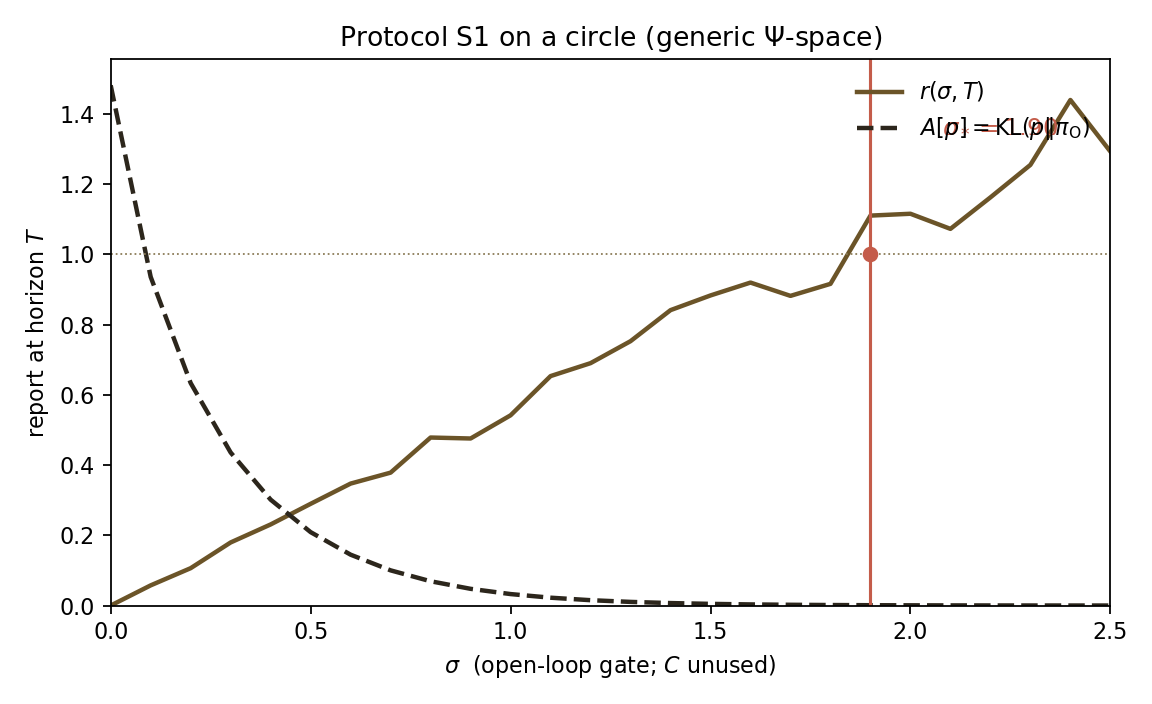
\includegraphics[width=0.88\linewidth]{../fig/s1-sweep.png}
  \caption{Protocol~S1, open-loop. Illustrative, not a lab figure of the Hopf stage.
  Space: the circle \(\mathbb{R}/(2\pi\mathbb{Z})\) (\(N=256\)).
  \(O=\partial_{\theta}\) (speed \(1\));
  \(\QC p=\piO-p\) with \(\piO\equiv 1/(2\pi)\)
  (rank-one jump to uniform, rate \(1\));
  \(T=2\), \(\varepsilon=10^{-12}\);
  initial \(p(\cdot,0)\) a bump at \(\pi\).
  Named alignment for this run:
  \(A[p]=\mathrm{KL}(p\Vert\piO)\) with \(\piO\) uniform.
  Life-drift \(D(\sigma,T)\) is not plotted; \(r(\sigma,T)\) and \(A[p]\) are.
  \(\sigma=0\) is pure transport; \(\sigma_{\ast}\) is where catalog jumps dominate.
  \(C\) is unused.}
  \label{fig:s1}
\end{figure}

\paragraph{Reading.}
Because S1 is open-loop, \(\sigma\) is the sweep parameter.
Jumps dominate when \(r(\sigma,T)\ge 1\).
Life-drift \(D(\sigma,T)=\mathrm{KL}(p_{T}^{\sigma}\Vert p_{T}^{0})\) grows.
The named \(A[p]=\mathrm{KL}(p\Vert\piO)\) drops because the catalog mixes
toward uniform.
This \(A\) is distance to the mixed state, not a target that restores the life shape.
A run that retunes \(\Op\), writes an equation for \(Z\),
or invents a third operator is not this protocol.

\paragraph{Out of scope.}
No \(350/\pi\), no Magic Islands, no pulsar coincidences,
no diffusion term, no Riemann examples.
Protocol~S2 is named above and not run.
